\documentclass[10pt,twocolumn]{article}
\usepackage{mla}
\usepackage{wrapfig}
\usepackage{amsmath}
\usepackage{hyperref}
\usepackage{graphicx}

\linespread{1}

\begin{document}
\begin{mla}{Paul}{English}{CHEM 1010-009}{Paul Neilson}{\today}{\textbf{Is There a Chemical Reaction Undergone When  Cooking Rice?}}


% What is happening to rice when it's cooked in water?
% - it's absorbing water like a sponge without a chemical reaction
% - it's undergoing a chemical reaction with water

% 1) based on your own personal observations pose a question you have
%    about the physical world around us. (describe how you made this
%    observation, and include a picture)
% 2) use your critical thinking and research skills to describe at least
%    two possible answers to your question.
% 3) choose one answer that makes sense to you.
% 4) show in a drawing, figure, diagram, or chemical reaction the
%    microscopic nature of matter related to your question.
% 5) describe why you favor your chosen hypothesis. use data and evidence
%    to support your idea (and make sure)
% 6) finally, you are welcome (but not required) to add a paragraph
%    describing the impact of your chosen technology on society

\section*{Observations}

Rice is a common food found in many kitchens and used across the world in many different meals. Rice is usually cooked at high temperatures for a period of time while submerged in water. During this time the rice kernels undergo a change in size and texture, making it larger and giving it a softer consistency. This can be seen in figure~\ref{fig:cooked_uncooked_rice}. The rice likely absorbs a portion of the water that it is cooked in. These observations may be consistent with a chemical reaction as defined in our textbook$^{8}$, although it could also be a physical change where the underlying structural makeup of the rice is not altered. 

\begin{figure}[h]
\centering
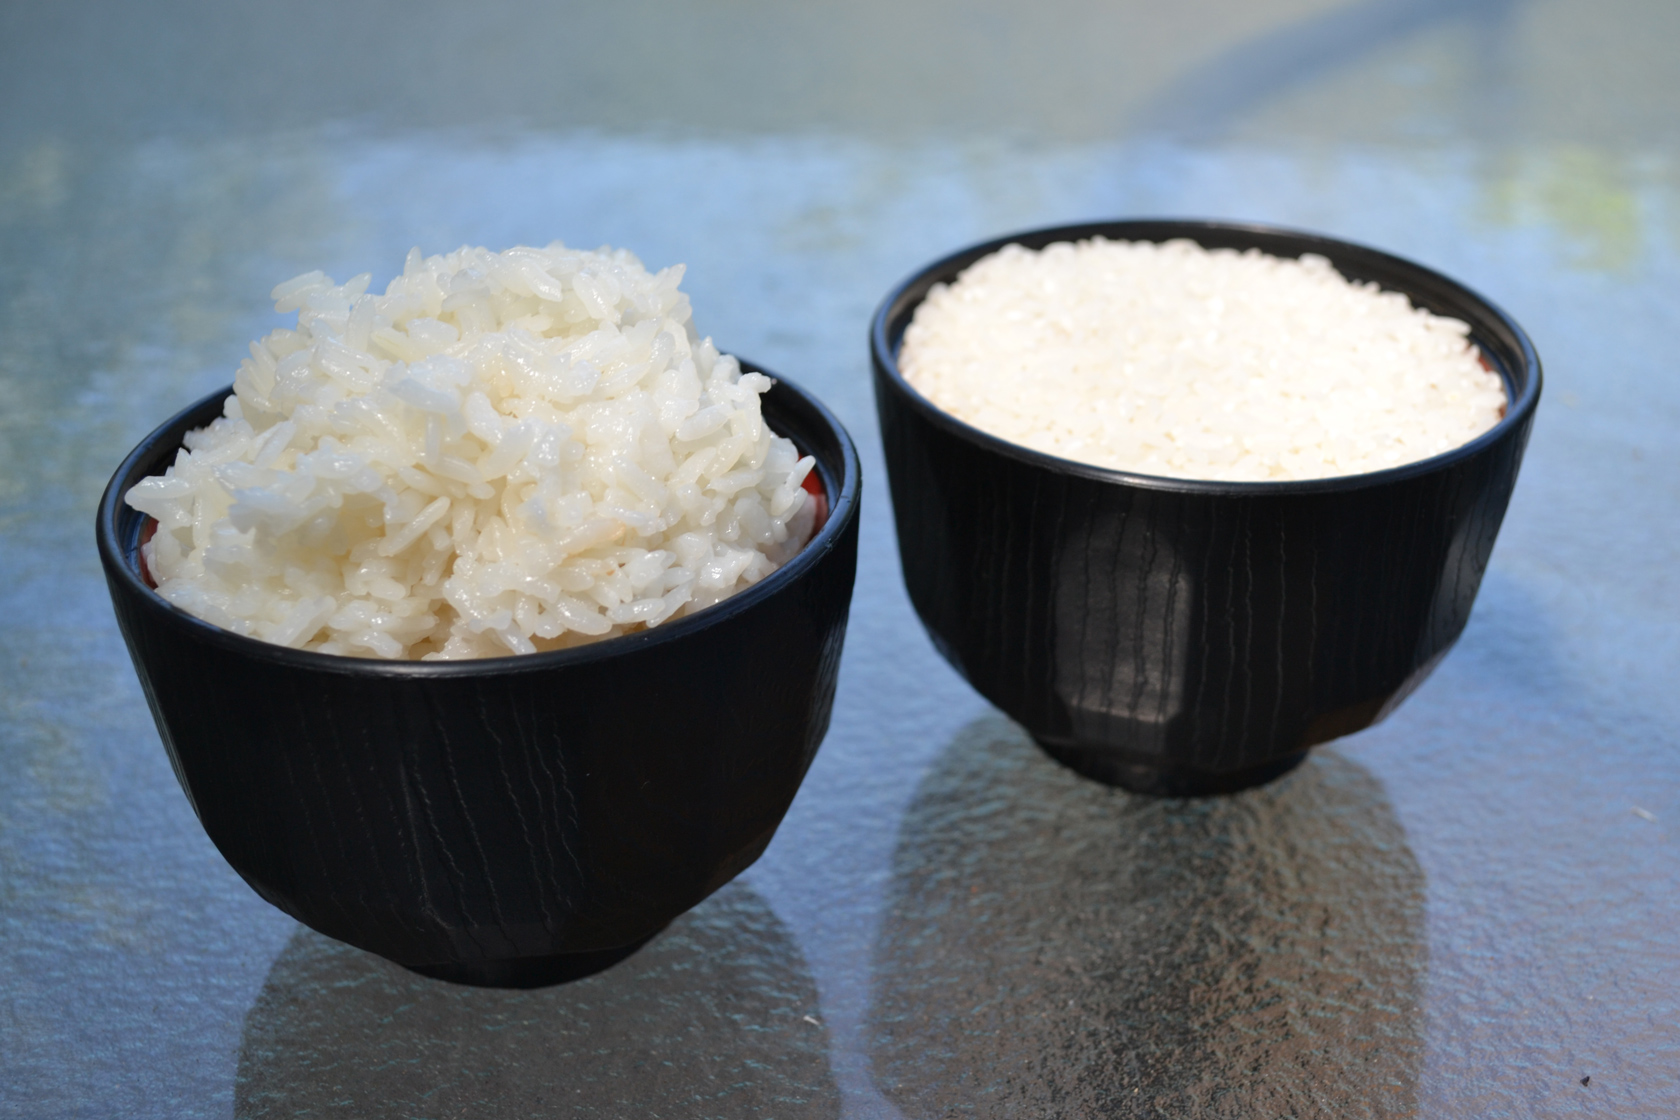
\includegraphics[width=\linewidth]{6740181017_5caf082268_o.jpg}
\caption{Comparison of cooked vs. uncooked rice. Cooked rice on the left.$^{6}$}
\label{fig:cooked_uncooked_rice}
\end{figure}


When cooking raw rice for 10 minutes we can measure a 2.5 times increase in volume, and up to 3.8 times increase with 20 minutes of cooking time.$^{3}$ After cooking, rice is usually stored in a cold environment to prevent bacterial growth that might be harmful or toxic to humans, not necessarily to prevent it from drying out. Rice will absorb water in lower temperatures over a longer timespan, similar to when heated. Heat acts as a catalyst, increasing the absorption of water, and speeding the change of rice properties. When left out after cooking rice seems to remain in it's post-cooked state rather than simply dry out and allowing it to be recooked. This would suggest that rather than simple physical change, the rice undergoes some kind of more intricate chemical change.

\section*{Starch Gelatinization}

Rice is primarily made up of simple carbohydrates, containing about 80g of carbohydrates in 100g of rice.$^4$
These rice carbohydrates are starches made up of amylose and amylopectin.$^7$
A starch is a polysaccharide, or long chain of sugar molecules.$^5$
Starch gelatinization is the reaction of a starch in water and heat. During gelatinization the starch molecule absorbs water which causes swelling and eventually breaks down the cell walls of the molecule. This process is permanent, and irreversible.$^1$ An example of the expanded molecular structure of the starches can be seen in figure~\ref{fig:starch_gelatinization}.

\begin{figure}[h]
\centering
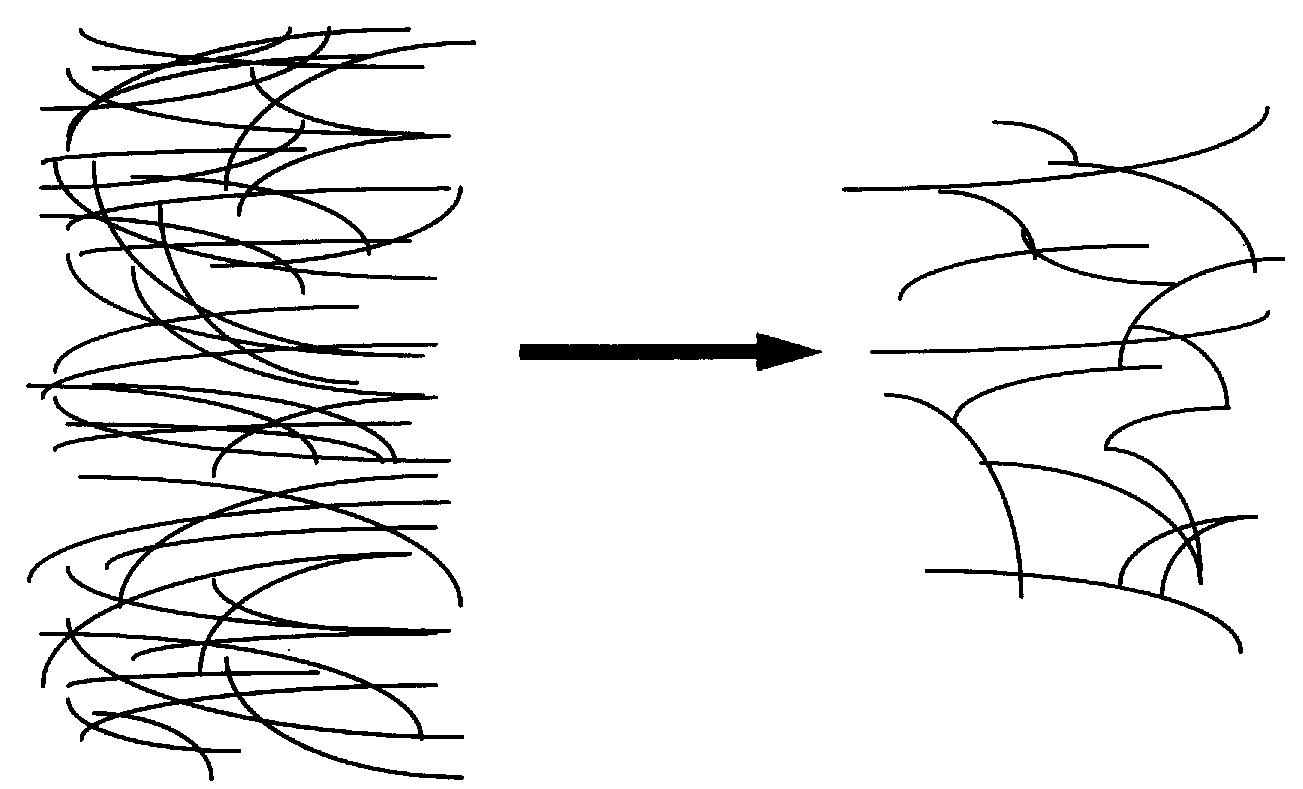
\includegraphics[width=\linewidth]{0170970201002.png}
\caption{Starch gelatinization at the molecular level.$^2$}
\label{fig:starch_gelatinization}
\end{figure}

This gelatinization is the chemical reaction that occurs in rice when we cook it. Which supports our chosen hypothesis of a chemical reaction rather than a physical change.

\begin{workscited}

\bibent
1. Hari, P. K., S. Garg, and S. K. Garg. ``Gelatinization of Starch and Modified Starch.'' \textit{Starch - St\"{a}rke} 41.3 (1989): 88-91. Print.

\bibent
2. Hart, Bob. ``Technology and Food Production.'' \textit{Nutrition \& Food Science} 97.2 (1997): 53-57. Emerald. Web. 06 Aug. 2013. $<$\href{http://www.emeraldinsight.com/journals.htm?articleid=866505}{http://www.emeraldinsight\dots}$>$.

\bibent
3. Kurien, P. P., R. Radhakrishna, H. S. R. Desikachar, and V. Subrahmanyan. ``Effect of Parboiling On The Swelling Quality of Rice.'' \textit{Cereal Chemistry} 41 (1964): 16-22. \textit{AACC International}. Web. 6 Aug. 2013. $<$\href{http://www.aaccnet.org/publications/cc/backissues/1964/Documents/chem41_16.pdf}{http://www.aaccnet.org/public\dots}$>$.

\bibent
4. ``Nutrient data laboratory''. \textit{United States Department of Agriculture}. Retrieved January 2012.

\bibent
5. P. Barham. ``The Science of Cooking''. Springer, 2001.

\bibent
6. Peter, Rowan. ``Compose a Photograph That Includes a `finished Product' and at Least One of Its `raw Materials'. Cooked Rice \& Uncooked Rice.'' \textit{Flickr}. Yahoo!, 22 Jan. 2012. Web. 06 Aug. 2013. $<$\href{http://www.flickr.com/photos/rowan_peter/6740181017/}{http://www.flickr.com/photos\dots}$>$.

\bibent
7. Zhong, Fang, Wallace Yokoyama, Qian Wang, and Charles F. Shoemaker. ``Rice Starch, Amylopectin, and Amylose:  Molecular Weight and Solubility in Dimethyl Sulfoxide-Based Solvents.'' \textit{Journal of Agricultural and Food Chemistry} 54.6 (2006): 2320-326. Print.

\bibent
8. Zumdahl, Steven S., and Donald J. DeCoste. ``Chapter 6.'' \textit{Introductory Chemistry: A Foundation}. 7th ed. Mason, OH: Cengage Learning, 2011. 145-46. Print.

\end{workscited}

\end{mla}
\end{document}

